\subsubsection{Подходы к оптимизации}

Стандартным подходом в оптимизации деревьев является pattern-matching \cite{pattern}. В простейшем случае это означает поддержку стека вершин. В ходе оптимизации вершины извлекаются из стека, локальная конфигурация вокруг вершины пробегает варианты оптимизаций, в случае успеха некоторые вершины сливаются и новые помещаются в стек.

Проблема такого подхода в графах обработки данных состоит в следующем. Если извлекать вершины из стека в произвольном порядке, можно получить ситуацию, при которой после оптимизаций в графе возникает петля (рис~\ref{fig:loop}). Это нарушает его корректность, данные для операции не готовы, т.к. чтобы их приготовить нужно запустить эту же операцию.

\begin{figure}[h]
    \centering
    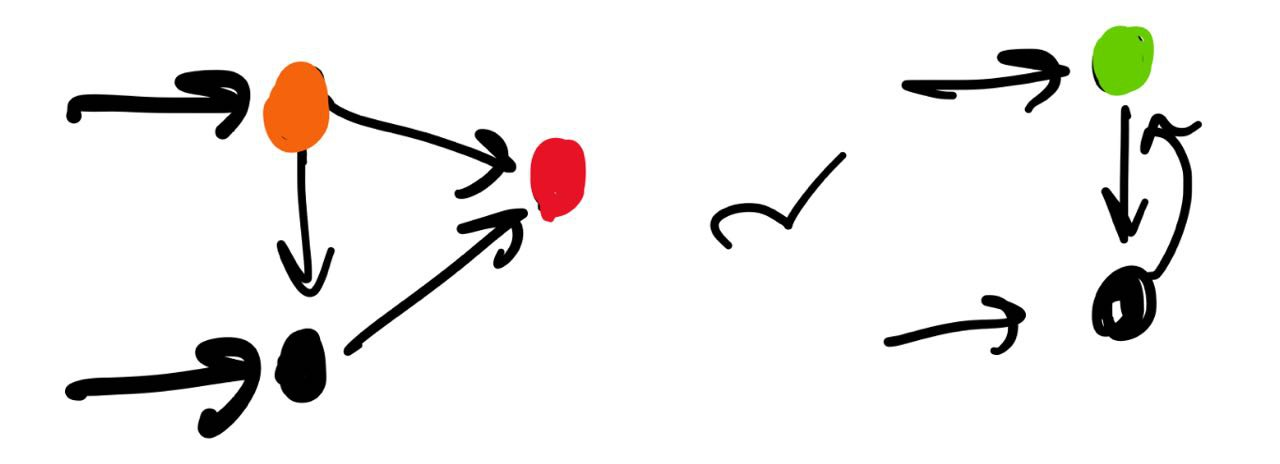
\includegraphics[width=0.5\textwidth]{img/loop.jpeg}
    \caption{Случай появления петли в графе}
    \label{fig:loop}
\end{figure}

Предлагается обходить граф, сохраняя зависимости по данным при обходе и в процессе оптимизаций. Это можно сделать с помощью обхода в топологическом порядке \cite{flume}. Для предложенного в данной работе алгоритма требуется более сильное упорядочивание вершин.
